% Fig. 1: pipeline overview. Compile standalone:  pdflatex fig1_overview.tex
\documentclass[tikz,border=2pt]{standalone}
\usepackage{times}
\usetikzlibrary{arrows.meta,positioning,calc,fit,backgrounds}
\begin{document}
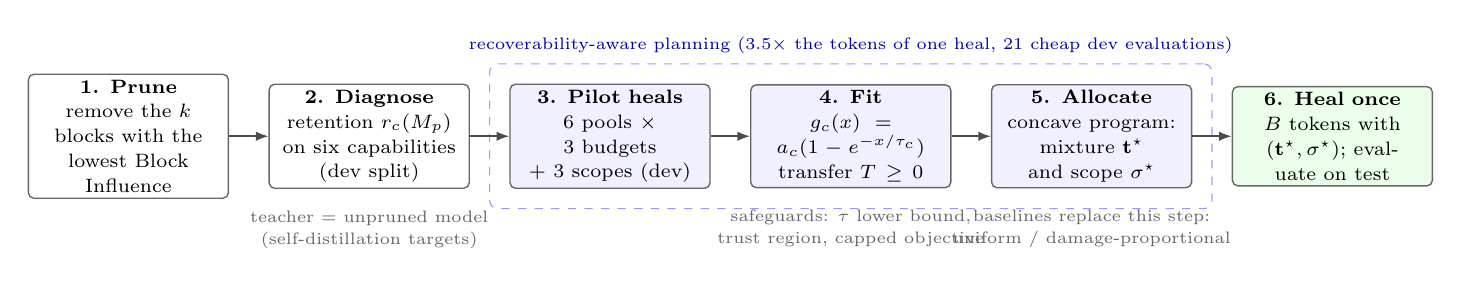
\begin{tikzpicture}[
  font=\fontsize{7.5}{9}\selectfont,
  box/.style={draw=black!60, line width=0.5pt, rounded corners=2pt, align=center, minimum height=9mm, text width=24mm, inner sep=2pt, fill=white},
  pilot/.style={box, fill=blue!6},
  outbox/.style={box, fill=green!8},
  arr/.style={-{Latex[length=1.6mm]}, line width=0.6pt, color=black!70},
  lab/.style={font=\fontsize{6.5}{8}\selectfont, color=black!60, align=center}
]
\node[box] (prune) {\textbf{1. Prune}\\remove the $k$ blocks with the lowest Block Influence};
\node[box, right=5mm of prune] (diag) {\textbf{2. Diagnose}\\retention $r_c(M_p)$ on six capabilities (dev split)};
\node[pilot, right=5mm of diag] (pil) {\textbf{3. Pilot heals}\\6 pools $\times$ 3 budgets\\+ 3 scopes (dev)};
\node[pilot, right=5mm of pil] (fit) {\textbf{4. Fit}\\$g_c(x)=a_c(1-e^{-x/\tau_c})$\\transfer $T\ge 0$};
\node[pilot, right=5mm of fit] (alloc) {\textbf{5. Allocate}\\concave program: mixture $\mathbf{t}^\star$ and scope $\sigma^\star$};
\node[outbox, right=5mm of alloc] (heal) {\textbf{6. Heal once}\\$B$ tokens with $(\mathbf{t}^\star,\sigma^\star)$; evaluate on test};
\draw[arr] (prune) -- (diag);
\draw[arr] (diag) -- (pil);
\draw[arr] (pil) -- (fit);
\draw[arr] (fit) -- (alloc);
\draw[arr] (alloc) -- (heal);
\node[lab, below=1.5mm of diag] {teacher = unpruned model\\(self-distillation targets)};
\node[lab, below=1.5mm of fit] {safeguards: $\tau$ lower bound,\\trust region, capped objective};
\node[lab, below=1.5mm of alloc] {baselines replace this step:\\uniform / damage-proportional};
\begin{scope}[on background layer]
  \node[draw=blue!40, dashed, rounded corners=3pt, inner sep=2.5mm, fit=(pil)(fit)(alloc), label={[lab, color=blue!70!black]above:recoverability-aware planning (3.5$\times$ the tokens of one heal, 21 cheap dev evaluations)}] {};
\end{scope}
\end{tikzpicture}
\end{document}
